\section{Framework and API}
The developer has a training dataset $D$ that consists of tuples of features $x_i$ and labels $y_i$ (either categorical or real-valued). She applies some function to this dataset $\textsf{train}(D)$, and returns a model $\textsf{model}(\cdot)$. Given a new $x_{new}$ this model returns a prediction $\hat{y}_{new}$:
\[
\hat{y}_{new} = \textsf{model}(x_{new})
\]

\vspace{0.5em}\noindent \textbf{Example Insurance Fraud Detection: } Consider the following running example of car insurance fraud detection. The training dataset $D$ has the following schema:
\[
\texttt{D(model, amount, at\_fault, description, fraud?)}
\]
where \texttt{model} is a categorical attribute describing the model of the car, \texttt{amount} is a double-valued amount that the person is claiming, \texttt{at\_fault} is a boolean variable describing whether the claimant is at fault, \texttt{description} is a string-valued attribute describing the nature of the claim, and \texttt{fraud?} is the yes/no label if the claim is fraudulent.

The function $\textsf{model}(\cdot)$ takes in a new unlabeled tuple:
\[
x_{new} = \texttt{r(model, amount, at\_fault, description, \_)}
\]
and predicts:
\[
\texttt{r(model, amount, at\_fault, description,} \hat{y}_{new} )
\]

\subsection{Challenges in Debugging}
Suppose $\textsf{model}(\cdot)$ issues an incorrect prediction and erroneously flags a fraudulent claim as not fraudulent. The data scientist is now tasked with debugging the model to understand why this error happened. 
She considers three possibilities: 
\begin{itemize}
\item \emph{(P1) Model Error.} The model is not sufficiently accurate enough to predict all claims correctly and needs to be tuned to err on the side of false positives.
\item \emph{(P2) Approximation Error.} The model was not trained with sufficient examples that look like $x_{new}$, and therefore, is not accurate in that region of the feature space.
\item \emph{(P3) Data Error.} The record $x_{new}$ is not consistent with respect to the training data, i.e., it represents the same information differently--leading to an unpredictable featurization.
\end{itemize}
The challenge for the data scientist is to determine which of these categories of errors best describes why the claim was mispredicted.
Intuitively, her process is to look at how ``similar'' tuples in the training dataset were predicted and compare to the given record. This will allow her to evaluate whether the problem is inherent to the model class or due to a fault of the training dataset or data processing pipeline. 

Existing approaches: 
\begin{itemize}
\item \emph{(S1) Nearest Neighbors. } The data scientist can search for the k nearest neighbors in the training dataset and use those as a guide.

\item \emph{(S2) Use A Simpler Model.} The data scientist can use any number of techniques to use the interpretable model from the start, then apply her domain expertise to understand why an error occurred.
\end{itemize}

The problem with (S1) and (S2) is that the models that are needed for such decision problems are necessarily complex. In the running example, there is a textual field \textsf{description}, which might be a very valuable feature for predicting fraud. Processing such data may require several NLP steps like a word-embedding, stop word removal, bi-gram featurization etc. So by design the feature space is complex and may not be interpretable by anyone other than an expert, and using a simpler model may not achieve the desired accuracy. Furthermore, as we move to a world where highly deep expressive models, which in principle can learn any deterministic function, it is well-known that these models have adversarial examples (i.e., imperceptible perturbations to the features that cause a change in prediction) \cite{szegedy2013intriguing}. This makes approaches like a nearest neighbor approach unreliable or even misleading. The approach that we propose identifies records that the classifier treats as similar, not just similarity in the feature space.

\subsection{Towards Debuggable Surrogates}
Let us consider the following working definition.
Debuggability is a measure of how well can we isolate tuples in the training dataset that significantly contributed to the prediction $ \hat{y}_{new}$.
We explore whether we given $\textsf{model}(\cdot)$ can train a surrogate model $\textsf{smodel}(\cdot)$ that approximates the original model, but is more debuggable.
One can think of a complex model as a collection of more compartmentalized models (ones that only apply to certain types of examples), and a meta model that selects which one of the sub-models is relevant to the example at hand.

This is a piecewise approximation of a complex function and by changing the allowed class models for the submodels and metamodel, we can get different behavior. 
As an illustrative example, consider when the meta model is much simpler.
For example, imagine if we hard-coded the following logic:
\begin{lstlisting}
def smodel(x):
    if amount > 10000:
    #one model for larger claims
        return submodel_1(x)
    elif a_fault:
    #one model for small at fault claims
        return submodel_2(x)
    else:
    #a default model
        return submodel_3(x)
\end{lstlisting}
Even though the logic that switches between the the submodels is simple (in fact it is a decision tree), the actual behavior is complex since the submodels encapsulate the complexity.
But, if we were to observe an anomaly, we would be able to precisely blame one of the submodels; thereby, getting a coarse predicate to select tuples that are assinged to that model.
there is an inherent tradeoff here where increasing the complexity of the meta-model improves the granularity of debugging, but potentially sacrifices on fidelity to the original model.

\subsection{Learning Meta Models} 
We propose an algorithm to automatically learn a meta-model and submodels from data to approximate the user's desired model.
This algorithm can run offline during the training phase and is generally no-more than a constant factor more expensive than standard model training
This algorithm is a special case of the algorithm, we proposed in prior work~\cite{DBLP:journals/corr/KrishnanGLMPG16, krishnan17}. At a high-level, the algorithm takes the dataset $D$ and the model \textsf{model} as input, and returns $\textsf{smodel}$, which consists of a decision-tree meta model that selects from a collection of $k$ submodels. Given a new record, the user can evaluate both:
\[
\hat{y}_{new} = \textsf{model}(x_{new})
\]
\[
\hat{y}_{new} = \textsf{smodel}(x_{new}) \approx \textsf{model}(x_{new})
\]
and use the structure of \textsf{smodel} to debug with knowledge that it approximates $\textsf{model}$.

\subsection{API and System}
We implemented this as a system in Python initially focusing on TensorFlow models.
For the user, the inputs are:
\begin{itemize}
\item \emph{Featurized Dataset. } The user provides a dataset of feature and label tuples.

\item \emph{Explainable Features. } The user lists a subset of features that are understandable.

\item \emph{Tensorflow Model Description. } The user provides a symbolic description of the model in Tensorflow.

\item \emph{Number of Sub-models. } The user provides the number of submodels to include in the surrogate model (denoted as $k$).
\end{itemize}

The output of the system is:
\begin{itemize}
\item \emph{Original Model. } The original model trained to completion

\item \emph{K Sub-Models. } The system returns K submodels trained on different partitions of the feature-space.

\item \emph{Decision Tree Meta Model. } The system returns a meta model that switches between the K submodels based on the input record.
\end{itemize}

We implemented the algorithm into a web interface that allows users to debug TensorFlow models Figure \ref{fig:interface}. The interface shows users mispredictions and allows them to search records that the classifier treats as similar.

\begin{figure*}[t]
    \centering
    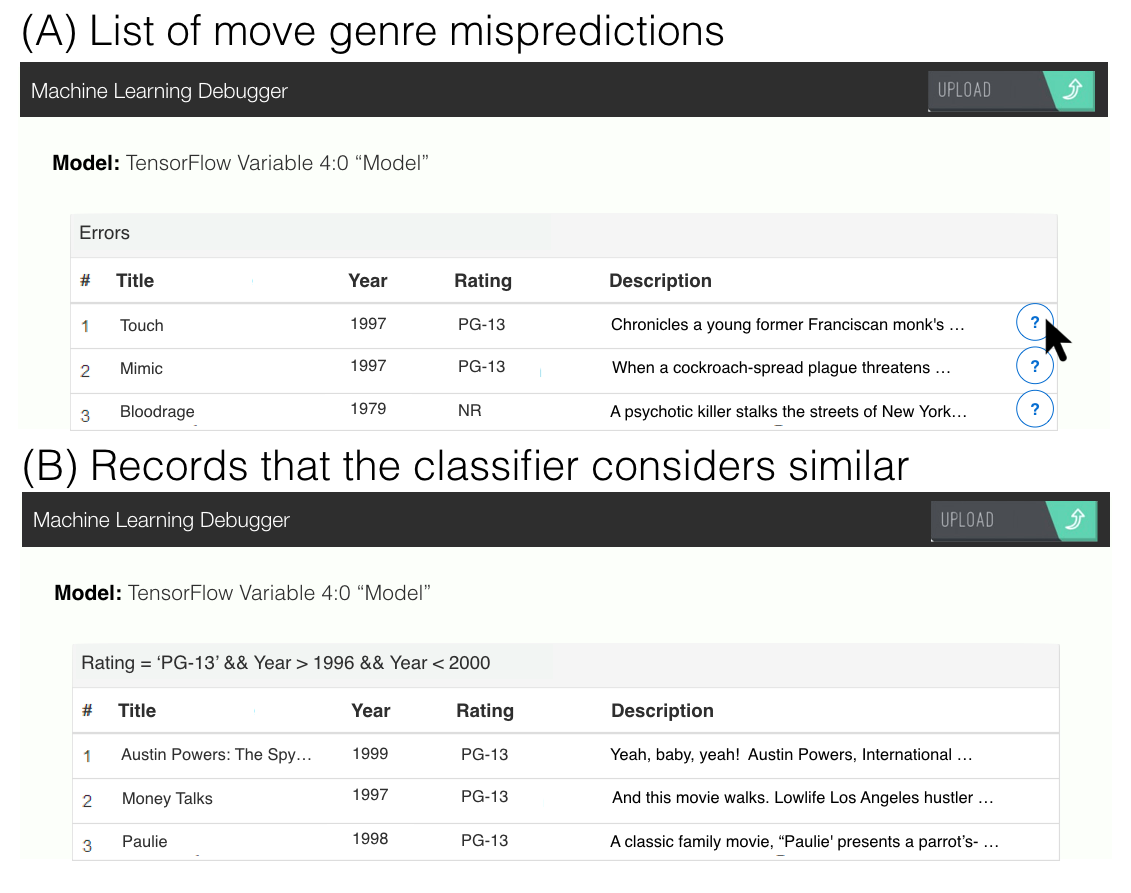
\includegraphics[width=0.6\textwidth]{figures/interface.png}
    \caption{A prototype interface implementing the algorithm. In (A), the interface lists a set tuples that were mis-predicted. Users can dig deeper by selecting one such tuple. (B) is the following panel which describes a predicate and records that the classifier considers as similar.}
    \label{fig:interface}
\end{figure*}